\documentclass[aip,jcp,reprint]{revtex4-2}
\usepackage{graphicx}    
\usepackage{chemformula}  
\usepackage{siunitx}      
\usepackage{pgfplots}
\usepgfplotslibrary{groupplots}
\pgfplotsset{compat=1.18}
\usepackage[utf8]{inputenc}
\usepackage[T1]{fontenc}
\usepackage[version=4]{mhchem}
\usepackage{amsmath,amssymb}
\usepackage{siunitx}
\sisetup{detect-all}
\usepackage{chemformula}
\usepackage{booktabs}
\usepackage{makecell}
\setlength{\tabcolsep}{3pt}
\usepackage{tikz}
\usetikzlibrary{arrows.meta,positioning}

\begin{document}

\title{Channel-Resolved Fourth-Order Vibrational Perturbation Theory for Quartic Centrifugal Distortion Constants}

\author{Vincenzo Barone}
\affiliation{INSTM, via G. Giusti 9, 50121 Firenze, Italy}
\email{vincebarone52@gmail.com}

\begin{abstract}

Quartic centrifugal distortion constants are essential parameters in the
analysis of high-resolution rotational spectra of polyatomic molecules.
Within the Watson rovibrational Hamiltonian these constants originate from
the coupling between rotational motion and vibrational displacements of
the molecular inertia tensor. While second-order vibrational perturbation
theory (VPT2) provides widely used expressions for the leading centrifugal
distortion terms, the quartic constants are often significantly affected
by higher-order anharmonic contributions. Despite this long-recognized
limitation, explicit working equations for quartic centrifugal distortion
constants at fourth perturbative order have not been systematically
developed because of the complexity of the Van Vleck contact transformation.

In the present work we introduce a channel-resolved formulation of
fourth-order vibrational perturbation theory for the quartic rotational
tensor. Instead of constructing the complete effective Hamiltonian through
a general Baker--Campbell--Hausdorff expansion, the quartic rotational block
is decomposed into physically distinct perturbative channels associated with
harmonic rovibrational coupling, quadratic inertia terms, mixed
cubic--rovibrational interactions, and cubic--cubic anharmonic couplings.
Each channel is derived and validated independently using exact symbolic
benchmarks obtained from a Van Vleck BCH engine for small-mode systems.

Within this decomposition the quartic VPT4 problem can be reorganized into
a standard first-level sector, explicit anharmonic extensions, and the first
controlled geometric breakdown associated with the quadratic-inertia channel.
In particular, the $H_{22}$ contribution is the first one that probes the
second response of the inverse inertia tensor and therefore the split
$\mu_2 = B(\mu_1) - N$, whereas the cubic--cubic channel $H_{30}H_{30}$
represents the dominant higher anharmonic contribution without being, by
itself, the first new geometric tensor level.

The most complex contribution arises from the cubic--cubic channel
$H_{30}H_{30}$. A systematic rank analysis of the full rotational scaffold
space shows that this contribution admits a minimal representation in terms
of seven independent rotational scaffold structures, providing the intrinsic
closure of the cubic--cubic channel at the level of the quartic rotational
tensor. This result replaces earlier gauge-based representations based on
over-compressed bases and yields a consistent multi-mode formulation.

The resulting equations therefore provide not only a practical route to the
evaluation of quartic centrifugal distortion constants at fourth perturbative
order, but also a tensor-hierarchical interpretation of how the VPT4 quartic
observable departs from the standard first-level closure.
An important conceptual consequence is that the present vibro-rotational
VPT4 problem differs structurally from the purely vibrational one. In the
latter, moving from VPT2 to VPT4 typically requires higher-order force-field
information and therefore probes the limits of a quartic force field. In the
present quartic rotational problem, by contrast, the fourth-order corrections
are generated by the cubic force field together with higher-order geometric
response terms of the inverse inertia tensor. Combined with analytic inertia
derivatives and molecular force-field data, the channel-resolved formulation
therefore enables efficient computation of quartic distortion constants for
polyatomic molecules while avoiding the combinatorial complexity of the full
BCH expansion.

\end{abstract}

\maketitle

\section{Introduction}

High-resolution rotational spectroscopy provides extremely accurate structural
information for isolated molecules and remains one of the most powerful tools
for probing molecular structure and intermolecular interactions.
\cite{BunkerJensen2005,Herzberg1945}
In modern spectroscopic analyses, rotational energy levels are commonly
described using effective Hamiltonians in which centrifugal distortion
constants account for the coupling between rotational and vibrational motion.
Among these parameters, the quartic centrifugal distortion constants
play a central role in reproducing high-$J$ rotational spectra of
polyatomic molecules.

From a theoretical perspective, centrifugal distortion arises from the
dependence of the molecular inertia tensor on vibrational motion.
Within the Watson rovibrational Hamiltonian, this coupling is naturally
described by expanding the Hamiltonian in normal coordinates and treating
vibrational effects perturbatively.
\cite{Watson1968,Watson1977,AlievWatson1976,Mills1972}
At second order in vibrational perturbation theory (VPT2), the leading
corrections to rotational constants and the associated quartic centrifugal
distortion terms can be derived in terms of first derivatives of the
inertia tensor with respect to the normal coordinates.
These expressions have been widely used in computational spectroscopy
and are implemented in several quantum-chemical programs.\cite{Franke2021,Gaw1991}

However, the second-order treatment is not always sufficient for the
quartic distortion constants.
In contrast to equilibrium rotational constants, which are often well
described at VPT2, quartic centrifugal distortion constants are known to
be significantly affected by higher-order anharmonic contributions.
This limitation has been recognized for a long time, and fourth-order
vibrational perturbation theory (VPT4) provides the natural framework
for improving the description.
Despite this, explicit working equations for quartic centrifugal
distortion constants at fourth perturbative order have not been
systematically developed in the literature.
The main obstacle lies in the rapid growth of the operator algebra
arising in the Van Vleck contact transformation of the rovibrational
Hamiltonian.\cite{VanVleck1932,Watson1968JCP}

It is important to stress that the present vibro-rotational VPT4 problem
differs in a fundamental way from the more familiar purely vibrational one.
In the vibrational case, moving from VPT2 to VPT4 typically introduces
higher-order force constants and therefore exposes the limits of a quartic
force field. For the quartic centrifugal distortion constants considered
here, by contrast, the fourth-order corrections arise from the cubic force
field together with higher-order geometric response terms of the inverse
inertia tensor. The problem is therefore not one of extending the potential
energy surface to arbitrarily high order, but of organizing in a controlled
way the interplay between cubic anharmonicity and higher-order inertia
response in the effective rotational block.

In the present work we revisit this problem using a channel-resolved
formulation of the perturbation expansion.
Rather than constructing the complete effective Hamiltonian through a
general Baker--Campbell--Hausdorff (BCH) expansion, we decompose the
quartic rotational block into physically distinct perturbative channels.
This approach exploits the natural structure of the Watson Hamiltonian
and allows each contribution to the quartic rotational tensor to be
derived and validated separately.\cite{Watson1967,Watson1968JCP}

The effective quartic rotational tensor can be written as a sum of
channel contributions originating from harmonic rovibrational coupling,
quadratic inertia terms, mixed cubic--rovibrational interactions, and
purely anharmonic cubic--cubic couplings.
The central point of the present work is that these channels should not
all be read on the same footing. In the tensorial interpretation
suggested by CeDiTT, the harmonic channel $H_{12}H_{12}$ defines the
standard first-level quartic sector generated by the first response of
the inverse inertia tensor. The mixed channel $H_{12}H_{30}$ then
provides the lowest explicit anharmonic extension of that same sector.
By contrast, the quadratic-inertia channel $H_{22}$ is the first one
that probes the second response of the inverse inertia tensor and
therefore the decomposition
\begin{equation}
\mu_2 = B(\mu_1) - N,
\end{equation}
where only $N$ corresponds to genuinely new intrinsic tensor content.
This makes $H_{22}$ the natural first controlled geometric breakdown of
the quartic first-level closure. The cubic--cubic channel $H_{30}H_{30}$
is finally the most intricate anharmonic contribution and the most
demanding one algebraically, but it should be kept conceptually
distinct from the first geometric breakdown.

A key result of the present work is that the cubic--cubic channel,
which represents the most complex contribution at fourth order,
admits a minimal representation in terms of seven independent
rotational scaffold structures.
This result emerges from a systematic rank analysis of the full
rotational scaffold space using exact symbolic benchmarks obtained
from a Van Vleck BCH engine for small-mode systems.

The resulting formulation provides a practical route to the evaluation
of quartic centrifugal distortion constants within a fourth-order
perturbative framework.
The theoretical structure is combined with a computational workflow
in which the individual perturbative channels are evaluated directly
from molecular force-field data and inertia derivatives.
In this way the expensive general BCH expansion is used only as a
benchmark tool, while the production calculations rely on a compact
channel-resolved representation of the quartic rotational tensor.

The present work therefore establishes a practical VPT4 framework for
quartic centrifugal distortion constants and clarifies the structural
roles of first-level closure, explicit anharmonic extension, and
controlled geometric breakdown in the quartic rotational tensor.
The formal development is accompanied by a symbolic implementation that
can be interfaced with molecular data from electronic-structure
calculations, enabling the routine evaluation of quartic distortion
constants for polyatomic molecules.

\section{Theory}

\subsection{Rovibrational Hamiltonian}

The starting point of the present formulation is the Watson rovibrational
Hamiltonian expressed in normal coordinates. In a perturbative expansion
around the equilibrium geometry, the Hamiltonian can be written as a sum
of operators classified by the order in vibrational coordinates and
rotational angular momentum operators,
\cite{Watson1968,Watson1977,AlievWatson1976}

\begin{equation}
H = H_{20} + H_{02} + H_{12} + H_{22} + H_{30} + H_{40} + \cdots ,
\end{equation}

where $H_{20}$ is the harmonic vibrational Hamiltonian,
$H_{02}$ is the rigid-rotor Hamiltonian, and the remaining terms
describe rovibrational couplings and anharmonic contributions.
The leading perturbative operators relevant for the present work are

\begin{align}
H_{12} &=
\frac{1}{2}
\sum_{\alpha\beta k}
\mu_{\alpha\beta,k}\,
q_k\,J_\alpha J_\beta ,
\\
H_{22} &=
\frac{1}{4}
\sum_{\alpha\beta kl}
\mu_{\alpha\beta,kl}\,
q_k q_l\,J_\alpha J_\beta ,
\\
H_{30} &=
\frac{1}{6}
\sum_{ijk}
\Phi_{ijk}\,
q_i q_j q_k ,
\\
H_{40} &=
\frac{1}{24}
\sum_{ijkl}
\Phi_{ijkl}\,
q_i q_j q_k q_l ,
\end{align}

where $q_i$ denote normal coordinates,
$J_\alpha$ are rotational angular momentum operators,
$\mu_{\alpha\beta,k}$ and $\mu_{\alpha\beta,kl}$ are first- and
second-order derivatives of the inverse inertia tensor with respect to
the normal coordinates, and $\Phi_{ijk}$ and $\Phi_{ijkl}$ are cubic and
quartic force constants.

The effective rovibrational Hamiltonian is obtained through a
Van Vleck contact transformation that eliminates vibrationally
off-diagonal terms order by order in perturbation theory.
The resulting effective Hamiltonian can be projected onto the
vibrational ground-state block to obtain an effective rotational
Hamiltonian.

\subsection{Quartic Rotational Tensor}

The quartic centrifugal distortion terms in the effective rotational
Hamiltonian can be written in terms of the quartic rotational tensor
$\tau_{\alpha\beta\gamma\delta}$ multiplying products of rotational
operators,

\begin{equation}
H_{\mathrm{quartic}} =
\tau_{xxxx} J_x^4
+
\tau_{yyyy} J_y^4
+
\tau_{zzzz} J_z^4
+
\tau_{xxyy} J_x^2 J_y^2
+
\tau_{xxzz} J_x^2 J_z^2
+
\tau_{yyzz} J_y^2 J_z^2 .
\end{equation}

It is convenient to collect the six independent components into the
vector

\begin{equation}
\bm{\tau} =
\begin{pmatrix}
\tau_{xxxx} \\
\tau_{yyyy} \\
\tau_{zzzz} \\
\tau_{xxyy} \\
\tau_{xxzz} \\
\tau_{yyzz}
\end{pmatrix}.
\end{equation}

These tensor elements represent the natural output of the perturbative
treatment before projection onto Watson's $A$- or $S$-reduced sets of
centrifugal distortion constants.\cite{Watson1968,Watson1977,Mills1972}

\subsection{Channel Decomposition of the Quartic Tensor}

Instead of constructing the complete effective Hamiltonian through a
general Baker--Campbell--Hausdorff expansion, we exploit the perturbative
structure of the Hamiltonian and decompose the quartic rotational tensor
into contributions arising from physically distinct perturbative
channels.

Up to fourth order in the perturbation expansion, the quartic rotational
tensor can be written as

\begin{equation}
\bm{\tau}^{(4)} =
\bm{\tau}^{(H_{12}H_{12})}
+
\bm{\tau}^{(H_{22})}
+
\bm{\tau}^{(H_{12}H_{30})}
+
\bm{\tau}^{(H_{30}H_{30})}
+
\bm{\tau}^{(H_{40})}.
\end{equation}

Each term corresponds to a well-defined perturbative mechanism:

\begin{itemize}
\item
$H_{12}H_{12}$ represents the harmonic rovibrational coupling arising
from first derivatives of the inertia tensor.
\item
$H_{22}$ corresponds to quadratic inertia contributions involving
second derivatives of the inertia tensor.
\item
$H_{12}H_{30}$ describes mixed interactions between cubic anharmonicity
and rovibrational coupling.
\item
$H_{30}H_{30}$ corresponds to purely anharmonic cubic--cubic
contributions.
\item
$H_{40}$ represents the quartic force-field term.
\end{itemize}

For the purposes of the present work, however, the channel decomposition
should be read not only as perturbative bookkeeping but as the first
appearance of a tensor hierarchy:

\begin{itemize}
\item
$\bm{\tau}^{(H_{12}H_{12})}$ defines the standard first-level quartic
sector generated by $\mu_1$.
\item
$\bm{\tau}^{(H_{12}H_{30})}$ is the lowest explicit anharmonic extension
of that same first-level structure.
\item
$\bm{\tau}^{(H_{22})}$ is the first channel that probes the second
geometric response and therefore the decomposition
$\mu_2 = B(\mu_1) - N$.
\item
$\bm{\tau}^{(H_{30}H_{30})}$ is the dominant higher anharmonic channel,
algebraically more complex than $H_{12}H_{30}$ but conceptually distinct
from the first geometric breakdown.
\end{itemize}

It is therefore useful to anticipate the hierarchical reading

\begin{equation}
\bm{\tau}^{(4)}
=
\bm{\tau}_{\mathrm{std}}
+
\bm{\tau}_{\mathrm{anh,std}}
+
\delta\bm{\tau}_{\mathrm{break}}
+
\bm{\tau}_{\mathrm{anh,high}},
\end{equation}

with
\begin{equation}
\bm{\tau}_{\mathrm{std}} = \bm{\tau}^{(H_{12}H_{12})},
\end{equation}
while the other terms will be identified more precisely below.

The perturbative channel structure of the quartic rotational tensor
and the minimal closure of the cubic--cubic contribution are summarized
schematically in Figure~\ref{fig:channels}.

\begin{figure*}[t]
\centering
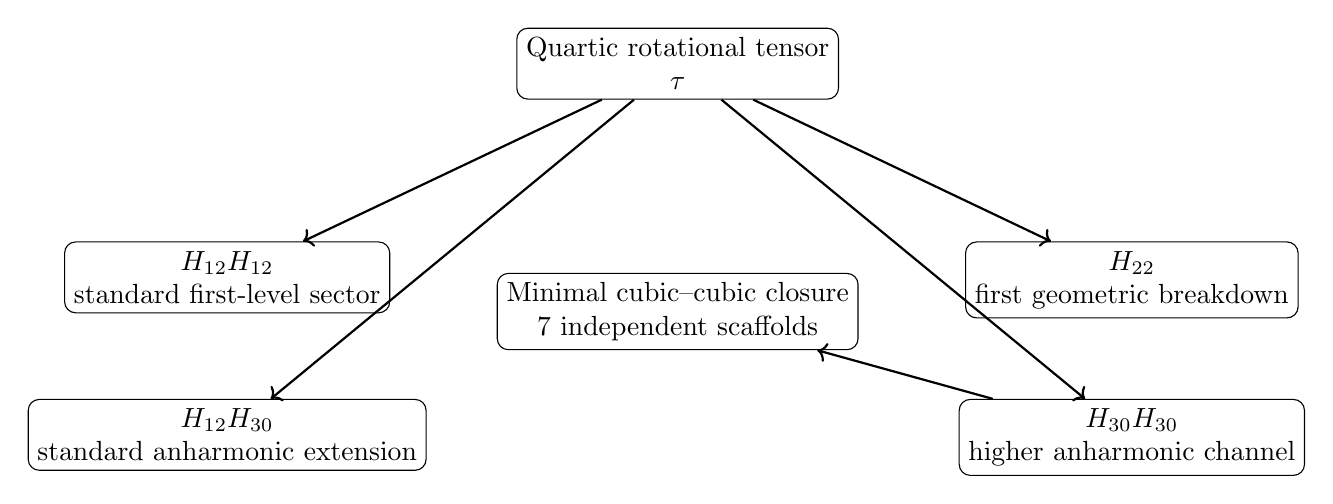
\begin{tikzpicture}[
node distance=2cm,
box/.style={rectangle,draw,rounded corners,align=center,minimum width=3.8cm,minimum height=0.9cm},
arrow/.style={->,thick}
]

\node[box] (tau)
{Quartic rotational tensor\\
$\bm{\tau}$};

\node[box,below left=1.8cm and 1.6cm of tau] (h12h12)
{$H_{12}H_{12}$\\
standard first-level sector};

\node[box,below right=1.8cm and 1.6cm of tau] (h22)
{$H_{22}$\\
first geometric breakdown};

\node[box,below of=h12h12] (h12h30)
{$H_{12}H_{30}$\\
standard anharmonic extension};

\node[box,below of=h22] (h30h30)
{$H_{30}H_{30}$\\
higher anharmonic channel};

\node[box,below=2.2cm of tau] (basis)
{Minimal cubic--cubic closure\\
7 independent scaffolds};

\draw[arrow] (tau) -- (h12h12);
\draw[arrow] (tau) -- (h22);
\draw[arrow] (tau) -- (h12h30);
\draw[arrow] (tau) -- (h30h30);
\draw[arrow] (h30h30) -- (basis);

\end{tikzpicture}

\caption{
Perturbative channel structure of the quartic rotational tensor.
The channels should be read not only as perturbative sources, but as
elements of a tensor hierarchy: $H_{12}H_{12}$ defines the standard
first-level sector, $H_{12}H_{30}$ its lowest explicit anharmonic
extension, $H_{22}$ the first controlled geometric breakdown, and
$H_{30}H_{30}$ the dominant higher anharmonic contribution. The
cubic--cubic channel admits a minimal closure in terms of seven
independent rotational scaffold structures.
}

\label{fig:channels}
\end{figure*}

\subsection{Vanishing of the Isolated Quartic Force-Field Channel}

An important simplification arises for the isolated quartic force-field
term. In the controlled limit

\begin{equation}
H = H_{20} + H_{02} + H_{40},
\end{equation}

the perturbation is purely vibrational and contains no rotational
operators. Consequently the Van Vleck transformation cannot generate
quartic rotational operators from $H_{40}$ alone, and the corresponding
contribution to the quartic rotational tensor vanishes,

\begin{equation}
\bm{\tau}^{(H_{40})} = \bm{0}.
\end{equation}

Therefore the quartic rotational tensor at fourth perturbative order is
completely determined by the remaining three perturbative channels,

\begin{equation}
\bm{\tau}^{(4)} =
\bm{\tau}^{(H_{12}H_{12})}
+
\bm{\tau}^{(H_{22})}
+
\bm{\tau}^{(H_{12}H_{30})}
+
\bm{\tau}^{(H_{30}H_{30})}.
\end{equation}

This point also highlights the difference between the present
vibro-rotational VPT4 problem and the purely vibrational one. In the
present quartic rotational tensor, no isolated quartic force-field channel
survives at the effective rotational level, so the fourth-order
corrections are governed by cubic-force and higher-order geometric
response terms rather than by an extension of the potential-energy
surface beyond the quartic force field for the observable itself.

In the following sections we analyze these contributions in detail,
with particular emphasis on the cubic--cubic channel $H_{30}H_{30}$,
which represents the most complex contribution to the quartic
rotational tensor.

\subsection{Hierarchical Interpretation of the Channel Decomposition}

The channel decomposition above is exact at the perturbative level, but
its physical interpretation is sharper when it is reorganized as a tensor
hierarchy.  The key point is that the four nonvanishing channels do not play
the same role.

The harmonic channel
\begin{equation}
\bm{\tau}^{(H_{12}H_{12})}
\end{equation}
defines the standard first-level quartic sector generated by the first
response of the inverse inertia tensor.  This is the direct quartic analogue
of the minimal CeDiTT sector already identified for standard quartic and
standard sextic centrifugal distortion.

The mixed channel
\begin{equation}
\bm{\tau}^{(H_{12}H_{30})}
\end{equation}
should then be read as the lowest explicit anharmonic extension of that same
first-level structure.  It dresses the standard quartic sector through the
cubic force field, but it does not by itself imply the appearance of a new
intrinsic geometric tensor level.

The quadratic-inertia channel
\begin{equation}
\bm{\tau}^{(H_{22})}
\end{equation}
is structurally special because it probes the second response of the inverse
inertia tensor.  In the tensor language used in the CeDiTT program, this
response is naturally decomposed as
\begin{equation}
\mu_2 = B(\mu_1) - N,
\end{equation}
where $B(\mu_1)$ is the bilinear closure generated algebraically from the
first-level object $\mu_1$, whereas $N$ is the first genuinely new intrinsic
geometric tensor.  For this reason $H_{22}$ is the natural candidate for the
first controlled geometric breakdown of the first-level quartic sector.

Finally, the cubic--cubic channel
\begin{equation}
\bm{\tau}^{(H_{30}H_{30})}
\end{equation}
represents a higher anharmonic contribution.  It is the most intricate
channel algebraically and often the most demanding one computationally, but
its complexity should not be conflated with the first geometric breakdown.
The distinction between explicit anharmonic complexity and genuinely new
geometric tensor content is one of the main organizing principles of the
present work.

In this sense the fourth-order quartic tensor is best read as
\begin{equation}
\bm{\tau}^{(4)}
=
\bm{\tau}_{\mathrm{std}}
+
\bm{\tau}_{\mathrm{anh,std}}
+
\delta\bm{\tau}_{\mathrm{break}}
+
\bm{\tau}_{\mathrm{anh,high}},
\label{eq:paper2_master_split}
\end{equation}
with
\begin{align}
\bm{\tau}_{\mathrm{std}} &= \bm{\tau}^{(H_{12}H_{12})}, \\
\bm{\tau}_{\mathrm{anh,std}} &= \bm{\tau}^{(H_{12}H_{30})}, \\
\delta\bm{\tau}_{\mathrm{break}} &\subset \bm{\tau}^{(H_{22})}, \\
\bm{\tau}_{\mathrm{anh,high}} &= \bm{\tau}^{(H_{30}H_{30})}.
\end{align}
Equation~\eqref{eq:paper2_master_split} is not a new perturbative identity;
it is the hierarchical reading of the exact channel decomposition that will
guide the remainder of the paper.

\section{Structure of the Cubic--Cubic Channel}

Among the perturbative contributions entering the quartic rotational tensor,
the cubic--cubic channel $H_{30}H_{30}$ represents the most complex
component of the fourth-order expansion.
This contribution originates from the coupling of two cubic anharmonic
terms through the Van Vleck contact transformation and therefore depends
quadratically on the cubic force constants $\Phi_{ijk}$.

\subsection{Rotational Scaffold Space}

The cubic--cubic contribution generates quartic products of rotational
operators through the interaction of the cubic force field with
rovibrational couplings.
Before projection onto the reduced rotational operator basis,
these contributions can be organized in terms of a set of rotational
scaffold structures.
Each scaffold corresponds to a distinct contraction pattern between
the cubic force constants and the rovibrational inertia derivatives.

In the present implementation the full cubic--cubic rotational scaffold
space is generated explicitly and contains 24 candidate structures.
These scaffolds represent all possible rotational contributions that
can arise from the cubic--cubic perturbative channel prior to the
imposition of linear relations between them.

\subsection{Rank Analysis}

To determine the intrinsic dimension of the cubic--cubic contribution,
we performed a systematic rank analysis of the scaffold space using
exact symbolic benchmarks obtained from the Van Vleck BCH engine for
small-mode systems.
The analysis was carried out independently for all components of the
quartic rotational tensor.

The resulting coefficient matrices exhibit a stable rank equal to seven
for every tensor component. This result demonstrates that the full
cubic--cubic contribution admits a minimal closure in terms of seven
independent scaffold structures. The appearance of a rank smaller than
the total number of candidate scaffolds reflects the existence of linear
relations between different contraction patterns of the cubic force
constants.

Importantly, the rank is found to be stable with respect to the number
of vibrational modes considered in the benchmark calculations,
indicating that the seven-dimensional scaffold space represents an
intrinsic property of the cubic--cubic perturbative channel rather
than an artifact of the reduced test systems.

\subsection{Minimal Cubic--Cubic Basis}

The pivot analysis of the scaffold matrices identifies a minimal set
of seven independent scaffold structures that span the cubic--cubic
contribution. These structures form a natural basis for expressing
the quartic rotational tensor arising from the $H_{30}H_{30}$ channel.

The cubic--cubic contribution can therefore be written as

\begin{equation}
\bm{\tau}^{(H_{30}H_{30})}
=
\sum_{r=1}^{7}
c_r^{(30,30)} \,
\bm{\mathcal{D}}_r ,
\end{equation}

where $\bm{\mathcal{D}}_r$ denote the seven rotational scaffold
structures and $c_r^{(30,30)}$ are coefficients depending on
the cubic force constants and harmonic frequencies.

This seven-scaffold representation replaces earlier formulations based
on smaller scaffold sets that suggested the presence of a gauge freedom
in the cubic--cubic channel. The rank analysis shows instead that the
correct closure of the cubic--cubic contribution requires a
seven-dimensional basis, eliminating the apparent gauge ambiguity.
In the hierarchical language of the present work, this rank-7 closure
should be read as the intrinsic closure of the higher anharmonic sector
$\bm{\tau}_{\mathrm{anh,high}}$, not as the first appearance of a new
geometric tensor level.

\subsection{Structure of the Cubic--Cubic Contribution}

Within the minimal scaffold representation, the coefficients
$c_r^{(30,30)}$ depend only on the cubic force constants and harmonic
frequencies through contractions of the form

\begin{equation}
\frac{\Phi_{abc}\Phi_{def}}
{\omega_a \omega_b \omega_c}
\end{equation}

combined with the appropriate modal symmetry factors.
The resulting expressions naturally generate multi-mode contributions
involving up to three distinct vibrational indices.

The cubic--cubic channel therefore represents the genuine anharmonic
core of the fourth-order correction to the quartic rotational tensor.
Once expressed in the minimal scaffold basis, the contribution can be
evaluated efficiently for arbitrary polyatomic molecules without
constructing the full BCH expansion.
Its structural role is therefore complementary to that of $H_{22}$:
$H_{30}H_{30}$ organizes the dominant high-order anharmonic content,
whereas $H_{22}$ isolates the first controlled geometric breakdown.

In the following section we describe the symbolic implementation and
benchmark validation used to obtain the cubic--cubic scaffold basis
and the corresponding coefficient expressions.

\section{Symbolic Implementation}

The theoretical framework described above has been implemented in a
symbolic computational workflow designed to derive and validate the
fourth-order contributions to the quartic rotational tensor.
The implementation combines a general Van Vleck BCH engine with a
dedicated channel-based solver for practical calculations.

\subsection{Van Vleck BCH Engine}

A general symbolic engine was developed to perform the Van Vleck
contact transformation of the rovibrational Hamiltonian. The
implementation represents vibrational coordinates in terms of bosonic
creation and annihilation operators,
\cite{VanVleck1932,Watson1968JCP}

\begin{equation}
q_i = \sqrt{\frac{\hbar}{2\omega_i}} (a_i + a_i^\dagger),
\end{equation}

with canonical commutation relations

\begin{equation}
[a_i , a_j^\dagger] = \delta_{ij}.
\end{equation}

Rotational operators $J_x$, $J_y$, and $J_z$ are treated as
non-commuting symbols.
The code implements operator multiplication, commutators, and recursive
bosonic normal ordering in order to evaluate the Baker--Campbell--Hausdorff
series

\begin{equation}
K = e^S H e^{-S},
\end{equation}

where the generator $S$ removes vibrationally off-diagonal terms order
by order in perturbation theory.

After normal ordering, the effective Hamiltonian is projected onto the
vibrational ground-state block,

\begin{equation}
H_{\mathrm{eff}} = \langle 0 | K | 0 \rangle ,
\end{equation}

and the quartic rotational block is extracted.

Although the BCH engine provides a formally exact symbolic
representation of the perturbation expansion, its direct application
to systems with several vibrational modes becomes computationally
expensive at fourth perturbative order.
For this reason the BCH engine is used primarily as a reference tool
for generating exact symbolic benchmarks for small-mode systems.

\subsection{Channel-Based Solver}

For practical calculations we employ a channel-resolved solver that
evaluates the individual perturbative contributions to the quartic
rotational tensor directly.
This implementation exploits the decomposition

\begin{equation}
\bm{\tau}^{(4)} =
\bm{\tau}^{(H_{12}H_{12})}
+
\bm{\tau}^{(H_{22})}
+
\bm{\tau}^{(H_{12}H_{30})}
+
\bm{\tau}^{(H_{30}H_{30})}.
\end{equation}

Each channel is implemented through explicit formulas derived from the
perturbative structure of the Hamiltonian.
This strategy avoids the combinatorial growth of the BCH series while
retaining the exact operator structure of the theory.

At the same time, the solver is not intended as a flat sum of unrelated
channels. Its purpose is to expose the hierarchical organization of the
quartic VPT4 observable. In practice, the implementation separates:

\begin{itemize}
\item the standard first-level quartic sector carried by
      $H_{12}H_{12}$;
\item the lowest explicit anharmonic extension carried by
      $H_{12}H_{30}$;
\item the first controlled geometric breakdown carried by the
      quadratic-inertia sector $H_{22}$;
\item the higher anharmonic channel $H_{30}H_{30}$, which is treated
      independently because of its distinct algebraic structure.
\end{itemize}

This organization is important conceptually and computationally. It
ensures that the implementation does not merely reproduce the full VPT4
quartic tensor, but also identifies which part of that tensor belongs to
the first-level closure already known from lower-order theory, which
part corresponds to explicit anharmonic dressing of that closure, and
which part represents the first genuinely new geometric information.

The harmonic channel $H_{12}H_{12}$ and the quadratic inertia channel
$H_{22}$ can be evaluated directly from analytic expressions involving
the inertia derivatives $\mu_{\alpha\beta,k}$ and
$\mu_{\alpha\beta,kl}$.
The mixed cubic--rovibrational channel $H_{12}H_{30}$ is implemented
through modal invariants constructed from the cubic force constants
and the rovibrational couplings.
In the hierarchical reading adopted here, this channel is not interpreted
as a new geometric tensor level. It is instead the lowest explicit
anharmonic dressing of the first-level quartic structure already carried
by $H_{12}H_{12}$.

The cubic--cubic channel $H_{30}H_{30}$ is evaluated using the minimal
seven-scaffold representation described in the previous section.
The coefficients of the scaffold structures are obtained from symbolic
benchmarks generated by the BCH engine and then used as closed-form
expressions in the channel solver.

The overall computational workflow is summarized in
Figure~\ref{fig:workflow}.

\begin{figure}[t]
\centering
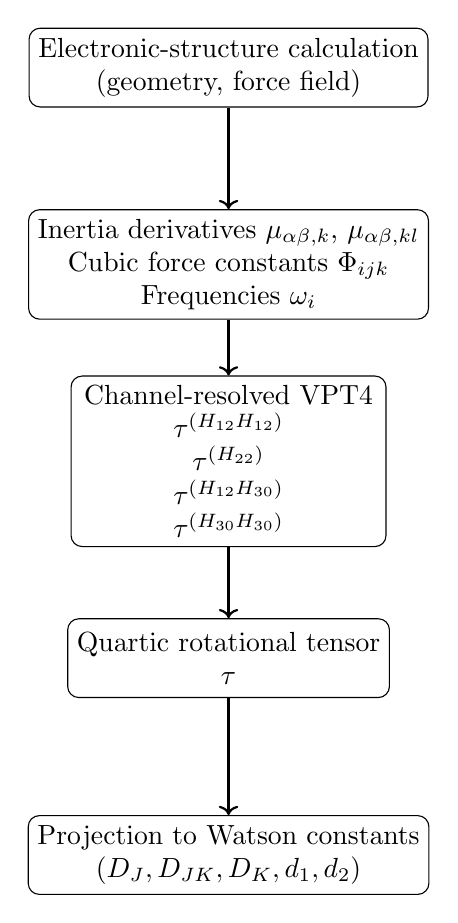
\begin{tikzpicture}[
node distance=2.5cm,
box/.style={rectangle,draw,rounded corners,align=center,minimum width=4cm,minimum height=1cm},
arrow/.style={->,thick}
]

\node[box] (gauss)
{Electronic-structure calculation\\
(geometry, force field)};

\node[box,below of=gauss] (inputs)
{Inertia derivatives $\mu_{\alpha\beta,k}$, $\mu_{\alpha\beta,kl}$\\
Cubic force constants $\Phi_{ijk}$\\
Frequencies $\omega_i$};

\node[box,below of=inputs] (channels)
{Channel-resolved VPT4\\
$\tau^{(H_{12}H_{12})}$\\
$\tau^{(H_{22})}$\\
$\tau^{(H_{12}H_{30})}$\\
$\tau^{(H_{30}H_{30})}$};

\node[box,below of=channels] (tau)
{Quartic rotational tensor\\
$\bm{\tau}$};

\node[box,below of=tau] (watson)
{Projection to Watson constants\\
$(D_J,D_{JK},D_K,d_1,d_2)$};

\draw[arrow] (gauss) -- (inputs);
\draw[arrow] (inputs) -- (channels);
\draw[arrow] (channels) -- (tau);
\draw[arrow] (tau) -- (watson);

\end{tikzpicture}

\caption{
Schematic workflow of the channel-resolved VPT4 method developed in this work.
Electronic-structure calculations provide harmonic frequencies,
cubic force constants, and derivatives of the inverse inertia tensor.
These quantities are used to evaluate the individual perturbative
channels contributing to the quartic rotational tensor
$\bm{\tau}$, which is finally projected onto Watson centrifugal
distortion constants.
}

\label{fig:workflow}
\end{figure}

\section{Results and Benchmark Validation}

The correctness of the formulation was assessed through
a series of symbolic benchmark calculations designed to reproduce the
quartic rotational tensor obtained from the full Van Vleck BCH expansion.
These benchmarks were performed for systems with increasing numbers of
vibrational modes in order to verify both the perturbative structure of
the individual channels and the multi-mode behavior of the cubic--cubic
contribution.

At the same time, the benchmarks have a second role. They do not merely
check that the channel-based solver reproduces the BCH engine. They also
test the hierarchical reading proposed in the present work, namely that
the quartic VPT4 observable can be decomposed into:

\begin{itemize}
\item a standard first-level baseline;
\item a lowest explicit anharmonic extension of that baseline;
\item a first controlled geometric breakdown;
\item and higher anharmonic channels.
\end{itemize}

From this point of view, the benchmarks should be read not only as
numerical validations, but also as structural tests of the tensor
hierarchy carried by the quartic rotational tensor.

\subsection{One-Mode Benchmark}

The one-mode system provides the simplest nontrivial test of the
implementation.
In this case the cubic force field contains a single element
$\Phi_{111}$ and the inertia derivatives reduce to single-mode
quantities.

The channel-resolved solver reproduces exactly the quartic rotational
tensor obtained from the BCH engine.
The resulting expressions separate naturally into symbolic families
associated with the different perturbative channels,
including contributions proportional to

\begin{equation}
\mu_1^2, \qquad
\mu_2, \qquad
\mu_1 \Phi_3, \qquad
\Phi_3^2 ,
\end{equation}

corresponding respectively to the $H_{12}H_{12}$,
$H_{22}$, $H_{12}H_{30}$, and $H_{30}H_{30}$ channels.
The exact agreement between the two approaches confirms the
correctness of the channel decomposition in the simplest case.

At the same time, the one-mode benchmark already illustrates the
hierarchical distinction emphasized in the present work. The terms
proportional to $\mu_1^2$ define the first-level quartic baseline; the
mixed $\mu_1\Phi_3$ terms are the first explicit anharmonic dressing of
that baseline; the terms proportional to $\mu_2$ identify the first
place where the second geometric response enters; and the $\Phi_3^2$
terms represent the first purely anharmonic higher channel.

\subsection{Two-Mode Benchmark}

The two-mode system provides the first test of genuine multi-mode
effects.
Collapsed-coupling benchmarks were constructed in which the inertia
derivatives and cubic force constants are replaced by simplified
symbolic parameters while preserving the index structure of the
perturbative operators.

In this case the BCH engine produces a quartic rotational tensor
containing contributions involving mixed modal indices.
The channel-based solver reproduces these results exactly, confirming
that the decomposition

\begin{equation}
\bm{\tau}^{(4)} =
\bm{\tau}^{(H_{12}H_{12})}
+
\bm{\tau}^{(H_{22})}
+
\bm{\tau}^{(H_{12}H_{30})}
+
\bm{\tau}^{(H_{30}H_{30})}
\end{equation}

remains valid in the multi-mode regime.

An important result of the two-mode benchmark is that the cubic--cubic
channel cannot be reduced to a trivial scalar renormalization of the
harmonic $H_{12}H_{12}$ contribution.
Instead, the cubic--cubic terms generate distinct rotational structures
that must be treated independently.

The same benchmark also clarifies that multi-mode complexity alone does
not identify the first breakdown. In the present hierarchy the relevant
question is not whether a contribution is algebraically complicated, but
whether it introduces genuinely new geometric tensor content. The
two-mode results therefore support the distinction between the higher
anharmonic channel $H_{30}H_{30}$ and the structurally different
quadratic-inertia channel $H_{22}$.

\subsection{Three-Mode Structure of the Cubic--Cubic Channel}

The most revealing benchmarks are obtained for three vibrational modes.
In this case the cubic force field contains elements of the form
$\Phi_{iii}$, $\Phi_{iij}$, and $\Phi_{ijk}$, allowing the cubic--cubic
channel to generate contributions involving up to three distinct
vibrational indices.

The BCH engine confirms that the cubic--cubic channel produces
genuinely three-mode structures such as

\begin{equation}
iij\_jkk
\quad\text{and}\quad
ijk\_ijk,
\end{equation}

which cannot be reduced to combinations of lower-mode contributions.
These terms therefore represent intrinsic multi-mode effects of the
anharmonic cubic force field.

The scaffold analysis described above
shows that all cubic--cubic contributions generated by the BCH engine
are contained within the seven-dimensional scaffold space identified
through the rank analysis.
The channel solver reproduces these results exactly when expressed in
the minimal scaffold basis.

This result is important for the present hierarchy because it separates
two different kinds of complexity. On the one hand, the cubic--cubic
channel is intrinsically high-dimensional and requires its own minimal
closure. On the other hand, that closure does not by itself identify the
first new geometric tensor level. The benchmark therefore reinforces the
main conceptual point of the paper: higher anharmonic complexity and
first geometric breakdown are related but distinct notions.

\subsection{Validation of the Channel Formulation}

The benchmark calculations demonstrate that the
implementation reproduces the full BCH expansion for all tested
systems.
In particular, the cubic--cubic contribution generated by the channel
solver matches the exact symbolic expressions obtained from the BCH
engine, including the full multi-mode structure.

These results confirm that the channel-based formulation provides an
exact representation of the fourth-order perturbative corrections to
the quartic rotational tensor while avoiding the combinatorial growth
associated with the full BCH expansion.

Taken together, the benchmark calculations therefore validate two
claims simultaneously. First, they confirm the exactness of the
channel-resolved formulation with respect to the full BCH reference.
Second, they support the hierarchical reading of the quartic VPT4
observable in terms of a first-level baseline, explicit anharmonic
extensions, a first controlled geometric breakdown, and higher
anharmonic channels.

\subsection{Benchmark Molecules: \texorpdfstring{\ce{H2O}, \ce{H2S}, \ce{H2CO}, and \ce{H2CS}}{H2O, H2S, H2CO, and H2CS}}

The symbolic benchmarks establish the formal correctness of the channel
decomposition, but they do not by themselves show how the hierarchy
behaves on real molecules.  For this reason we also interfaced the
present implementation with Gaussian-style quartic benchmark data for
\ce{H2O}, \ce{H2S}, \ce{H2CO}, and \ce{H2CS}, and compared the resulting
quartic constants with the VPT and PFIT/RVCI trends reported in
Ref.~\citenum{Dinu2022}.  Throughout this comparison all quartic
constants are considered in Watson's $S$ reduction, and the required
benchmark-consistent axis mapping is inferred directly from the
Gaussian quartic reference.

The first important result is that the standard quartic baseline is now
numerically under control for all four systems.  Once the benchmark
axis convention is enforced, the present order-2 implementation
reproduces the Gaussian quartic constants with sub-\si{kHz} residuals in
all cases.  This means that the remaining differences observed at
fourth order are not artifacts of the Watson projection or of the axis
assignment, but reflect the actual higher-order channel content of the
present implementation.

Table~\ref{tab:paper2_benchmark_summary} summarizes the numerical
diagnostic.  For \ce{H2CO} and \ce{H2CS} the dominant higher-order
correction comes from the mixed channel $H_{12}H_{30}$ and remains
moderate, shifting the quartic constants only by a few
\si{10^2}{kHz} at most.  This is consistent with the published VPT/PFIT-RVCI
comparison, where the quartic constants of formaldehyde and
thioformaldehyde already show only modest deviations at the VPT2
level.\cite{Dinu2022}

The situation is different for \ce{H2S}.  Here the standard quartic
benchmark is still reproduced essentially exactly at order 2, but the
largest fourth-order correction is no longer controlled by
$H_{12}H_{30}$.  Instead, the cubic--cubic channel $H_{30}H_{30}$
becomes dominant and changes the quartic constants on the
\si{10^5}{kHz} scale.  In the language of the present paper, this is a
case in which the higher anharmonic channel becomes numerically
important even though the first geometric breakdown channel $H_{22}$
remains small.

Water is the most revealing case.  The order-2 quartic benchmark again
matches the Gaussian reference once the benchmark axis convention is
used, but the fourth-order correction is dominated overwhelmingly by
$H_{30}H_{30}$ and drives the quartic constants far outside the scale of
the standard result.  This is precisely the molecule for which the
published VPT/VCI comparison shows that the quartic constants are most
problematic.\cite{Dinu2022}  In the present implementation, \ce{H2O}
therefore acts as a stress test: it does not merely show that
higher-order corrections matter, but indicates that the cubic--cubic
sector is the critical piece to be understood quantitatively before the
full VPT4 quartic model can be regarded as predictive.

\begin{table*}[t]
\centering
\caption{Diagnostic summary of the quartic benchmark calculations for
\ce{H2O}, \ce{H2S}, \ce{H2CO}, and \ce{H2CS}.  All quartic constants are
in Watson's $S$ reduction and expressed in kHz.  The quantity
$\max|\Delta_{\mathrm{std}}|$ is the maximum absolute deviation between
the present order-2 quartic constants and the Gaussian benchmark.  The
quantity $\max|\Delta_{\mathrm{VPT4}}|$ is the maximum absolute shift
between the present fourth-order total and the order-2 baseline over the
five quartic constants $(D_J,D_{JK},D_K,d_1,d_2)$.}
\begin{tabular}{lccc}
\toprule
Molecule & $\max|\Delta_{\mathrm{std}}|$ & Dominant higher-order channel & $\max|\Delta_{\mathrm{VPT4}}|$ \\
\midrule
\ce{H2O}  & 0.016 & $H_{30}H_{30}$ & $8.55\times 10^{6}$ \\
\ce{H2S}  & $4.3\times 10^{-4}$ & $H_{30}H_{30}$ & $2.54\times 10^{5}$ \\
\ce{H2CO} & $9.0\times 10^{-6}$ & $H_{12}H_{30}$ & $1.87\times 10^{2}$ \\
\ce{H2CS} & $2.1\times 10^{-4}$ & $H_{12}H_{30}$ & $1.26\times 10^{2}$ \\
\bottomrule
\end{tabular}
\label{tab:paper2_benchmark_summary}
\end{table*}

These four cases therefore play different roles.  \ce{H2CO} and
\ce{H2CS} are useful regular benchmarks that confirm the consistency of
the standard sector and the moderate size of the lowest explicit
anharmonic extension.  \ce{H2S} already shows that the higher
anharmonic channel can become numerically dominant.  \ce{H2O}, finally,
marks the regime in which the present fourth-order quartic problem
ceases to be a mild correction to the standard baseline and instead
becomes a genuine diagnostic of the limits of the perturbative
description itself.

\section{Interface with Gaussian and Final Projection to Watson Constants}
The VPT4 formulation developed in this work is intended to be interfaced
with molecular data obtained from electronic-structure calculations and
projected onto Watson quartic centrifugal distortion constants in a manner
consistent with Gaussian.\cite{Franke2021,Gaw1991}

\subsection{Required Molecular Data}
The program must read or reconstruct the following quantities:
\begin{enumerate}
\item harmonic vibrational frequencies $\omega_i$,
\item equilibrium geometry and atomic masses,
\item normal modes in a consistent mass-weighted convention,
\item cubic force constants $\Phi_{ijk}$,
\item first derivatives of the inverse inertia tensor,
\[
\mu_{\alpha\beta,i}
=
\left.
\frac{\partial (I^{-1})_{\alpha\beta}}{\partial Q_i}
\right|_0,
\]
\item second derivatives of the inverse inertia tensor,
\[
\mu_{\alpha\beta,ij}
=
\left.
\frac{\partial^2 (I^{-1})_{\alpha\beta}}{\partial Q_i \partial Q_j}
\right|_0.
\]
\end{enumerate}

Within the present operational VPT4 framework, quartic force constants are not required as independent input for the quartic rotational tensor itself, because the isolated $H_{40}$ channel does not generate quartic rotational operators.

The quartic rotational tensor is evaluated as
\[
\bm{\tau}
=
\bm{\tau}^{(12,12)}
+
\bm{\tau}^{(22)}
+
\bm{\tau}^{(12,30)}
+
\bm{\tau}^{(30,30)},
\]
with
\[
\bm{\tau}^{(40)} = \bm{0}.
\]
The required molecular data for each channel are:
\begin{itemize}
\item $H_{12}H_{12}$: $\omega_i$ and $\mu_{\alpha\beta,i}$,
\item $H_{22}$: $\omega_i$ and $\mu_{\alpha\beta,ij}$,
\item $H_{12}H_{30}$: $\omega_i$, $\mu_{\alpha\beta,i}$, $\mu_{\alpha\beta,ij}$, and $\Phi_{ijk}$,
\item $H_{30}H_{30}$: $\omega_i$, $\mu_{\alpha\beta,i}$, and $\Phi_{ijk}$.
\end{itemize}

The quartic rotational contribution is naturally represented in the compressed form
\[
(\tau_{xxxx},\tau_{yyyy},\tau_{zzzz},\tau_{xxyy},\tau_{xxzz},\tau_{yyzz}).
\]
For the quartic tensor derived in the present formulation, the allowed operator
structure implies pair--pair closure. As a consequence, the Gaussian-consistent
reduced matrix $\tau'_{ij}$ can be obtained directly from the compressed tensor,
without explicit reconstruction of a general Wilson four-index tensor. The
diagonal elements are
\[
\tau'_{xx}=\tau_{xxxx},\qquad
\tau'_{yy}=\tau_{yyyy},\qquad
\tau'_{zz}=\tau_{zzzz},
\]
whereas the mixed elements are
\[
\tau'_{xy}=\frac{1}{2}\tau_{xxyy},\qquad
\tau'_{xz}=\frac{1}{2}\tau_{xxzz},\qquad
\tau'_{yz}=\frac{1}{2}\tau_{yyzz}.
\]
The Cartesian quartic matrix is then defined as
\[
T_{ij}=\tau'_{ij}/4.
\]

The cylindrical quartic quantities are
\begin{align}
T_{400} &= \frac{3T_{11}+3T_{22}+2T_{12}}{8},\\
T_{220} &= T_{13}+T_{23}-2T_{400},\\
T_{040} &= T_{33}-T_{220}-T_{400},\\
T_{202} &= \frac{T_{11}-T_{22}}{4},\\
T_{022} &= \frac{T_{13}-T_{23}}{2}-T_{202},\\
T_{004} &= \frac{T_{11}+T_{22}-2T_{12}}{16}.
\end{align}

\subsection{Practical Program Workflow}
A consistent implementation should proceed as follows:
\begin{enumerate}
\item read equilibrium geometry, atomic masses, harmonic frequencies, normal modes, and cubic force constants;
\item compute the first and second derivatives of the inverse inertia tensor from the equilibrium structure and the normal modes;
\item evaluate the perturbative channel contributions to the quartic rotational tensor;
\item assemble the full four-index quartic tensor $\tau_{ijkl}$;
\item build the reduced matrix $\tau'_{ij}$;
\item define $T_{ij}=\tau'_{ij}/4$;
\item apply the transformation defined above to obtain Watson quartic centrifugal distortion constants.
\end{enumerate}

In this workflow the derivatives of the inverse inertia tensor are not assumed as direct input data. Instead, they are determined
analytically from the molecular geometry, masses, and normal-mode displacements. This makes the procedure independent of any specific
electronic-structure output format and suitable for implementation with data obtained from different quantum-chemical programs.

\section{Conclusions}
In this work we have developed a channel-resolved formulation of
fourth-order vibrational perturbation theory for the evaluation of
quartic centrifugal distortion constants within the Watson rovibrational
Hamiltonian framework. The approach avoids the combinatorial complexity
of a full Baker--Campbell--Hausdorff expansion by decomposing the quartic
rotational tensor into physically distinct perturbative channels and
then reorganizing them into a tensor hierarchy.

Within this formulation the quartic rotational tensor naturally
decomposes into contributions arising from harmonic rovibrational
coupling ($H_{12}H_{12}$), quadratic inertia terms ($H_{22}$),
mixed cubic--rovibrational interactions ($H_{12}H_{30}$), and
cubic--cubic anharmonic couplings ($H_{30}H_{30}$).
The isolated quartic force-field term $H_{40}$ does not generate
quartic rotational operators and therefore does not contribute to the
quartic rotational tensor for the vibrational ground-state block.
This channel structure provides a transparent physical interpretation
of the different perturbative mechanisms contributing to centrifugal
distortion.

The main conceptual point of the present formulation is that the channel
decomposition should be read as a tensor hierarchy rather than as a flat
perturbative list. The $H_{12}H_{12}$ contribution defines the standard
first-level quartic sector, and the mixed channel $H_{12}H_{30}$ provides
its lowest explicit anharmonic extension. The $H_{22}$ contribution is
structurally special because it probes the second response of the inverse
inertia tensor and therefore the split $\mu_2 = B(\mu_1) - N$, where only
$N$ corresponds to genuinely new intrinsic tensor content. By contrast,
the cubic--cubic channel $H_{30}H_{30}$ is the most intricate anharmonic
contribution and the most demanding one algebraically, but it should be
kept conceptually distinct from the first controlled geometric breakdown.

Equation~\eqref{eq:paper2_master_split} provides the corresponding
hierarchical summary: a standard quartic baseline, a lowest explicit
anharmonic extension, a first controlled geometric breakdown, and higher
anharmonic channels that may be numerically important without being the first
new tensor level.

The practical consequence is that quartic VPT4 on the vibro-rotational side
should not be viewed simply as ``more perturbative channels'' than VPT2.  It
should instead be viewed as the first place where one can separate, within a
single observable, the first-level geometric closure from its lowest
anharmonic dressing and from the first irreducible geometric correction.

The most intricate contribution is associated with the cubic--cubic
channel $H_{30}H_{30}$. A systematic rank analysis of the full rotational
scaffold space shows that this channel admits a minimal closure in terms
of seven independent scaffold structures. This result clarifies the
structure of the higher anharmonic sector, replaces earlier
over-compressed representations that suggested an artificial gauge
freedom, and shows that the intrinsic closure of $H_{30}H_{30}$ is a
property of the anharmonic channel itself rather than of the first
geometric breakdown.

An important consequence of the present work is that the quartic
vibro-rotational VPT4 problem differs structurally from the purely
vibrational one. In the latter, fourth-order perturbation theory
typically requires higher-order force constants and therefore probes the
limits of a quartic force field. In the present quartic rotational
problem, however, the relevant fourth-order corrections are generated by
the cubic force field together with higher-order geometric derivatives of
the inverse inertia tensor. This makes the vibro-rotational VPT4
framework considerably more accessible in practice than a fully
analogous vibrational treatment.

The resulting channel-resolved equations therefore provide a practical
framework for evaluating quartic centrifugal distortion constants at
fourth perturbative order and, at the same time, for separating the
standard baseline, its explicit anharmonic dressing, and the first
irreducible geometric correction. In the computational workflow developed here,
the general Van Vleck BCH engine is used only to generate exact symbolic
benchmarks for small-mode systems, while the production calculations rely
on the direct channel formulation. This strategy preserves the formal
rigor of the perturbation theory while enabling efficient evaluation of
quartic distortion constants for polyatomic molecules.

The present work therefore establishes a practical VPT4 framework for
quartic centrifugal distortion constants and clarifies, at the level of
the quartic observable itself, the distinct structural roles of
first-level closure, explicit anharmonic extension, first controlled
geometric breakdown, and higher anharmonic complexity.
Future developments will focus on interfacing the channel-resolved
formulation with molecular force-field data obtained from
electronic-structure calculations, allowing routine evaluation of
quartic centrifugal distortion constants for realistic molecular systems,
and on projecting the resulting higher-order tensor hierarchy onto the
corresponding higher-order spectroscopic observables.


\appendix

\section{Quartic tensor definition}
The quartic centrifugal distortion block can be written as
\begin{equation}
H_{\mathrm{quartic}} = \tau_{xxxx} J_x^4 + \tau_{yyyy} J_y^4 + \tau_{zzzz} J_z^4
+ \tau_{xxyy} J_x^2 J_y^2 + \tau_{xxzz} J_x^2 J_z^2 + \tau_{yyzz} J_y^2 J_z^2.
\end{equation}
Collecting the surviving commuting monomials into the six-component vector
\begin{equation}
\bm{\tau} = (\tau_{xxxx},\tau_{yyyy},\tau_{zzzz},\tau_{xxyy},\tau_{xxzz},\tau_{yyzz})^T
\end{equation}
provides a convenient representation of the quartic tensor before projecting onto Watson's reduced constants.

\section{Channel decomposition and hierarchy}
The fourth-order tensor splits into the perturbative channels
\begin{equation}\label{eq:channel_sum}
\bm{\tau}^{(4)} = \sum_{\text{chan}} \bm{\tau}^{(\text{chan})} =
\bm{\tau}^{(H_{12}H_{12})}+\bm{\tau}^{(H_{22})}+\bm{\tau}^{(H_{12}H_{30})}+\bm{\tau}^{(H_{30}H_{30})}.
\end{equation}
This sum can be reorganized to emphasize the tensor hierarchy introduced in the main text:
\begin{equation}\label{eq:paper2_master_split}
\bm{\tau}^{(4)} = \bm{\tau}_{\mathrm{std}} + \bm{\tau}_{\mathrm{anh,std}}+\delta\bm{\tau}_{\mathrm{break}}+\bm{\tau}_{\mathrm{anh,high}}.
\end{equation}
The notation is chosen so that
\begin{align}
\bm{\tau}_{\mathrm{std}} &= \bm{\tau}^{(H_{12}H_{12})},\notag\\
\bm{\tau}_{\mathrm{anh,std}} &= \bm{\tau}^{(H_{12}H_{30})},\notag\\
\delta\bm{\tau}_{\mathrm{break}} &\subset \bm{\tau}^{(H_{22})},\notag\\
\bm{\tau}_{\mathrm{anh,high}} &= \bm{\tau}^{(H_{30}H_{30})}.
\end{align}
The quadratic-inertia channel thus isolates the first geometric breakdown carried by the intrinsic tensor $N$ in the decomposition
\begin{equation}
\mu_2 = B(\mu_1) - N,
\end{equation}
where $B(\mu_1)$ denotes the bilinear closure built from the first derivatives and $N$ represents the first genuinely new second-level tensor.

\section{Channel representations}
\subsection{$H_{12}H_{12}$ and $H_{12}H_{30}$}
The harmonic channel is generated by the first inertia derivatives
\begin{equation}
\tau^{(H_{12}H_{12})}_{\alpha\beta\gamma\delta} = -\frac{1}{8}\sum_k \frac{\mu_{\alpha\beta,k}\mu_{\gamma\delta,k}}{\omega_k^2},
\end{equation}
whereas the mixed cubic channel can be written as a linear combination of the modal invariants $S_1,S_2,S_3$ defined in the main text. It provides the lowest explicit anharmonic dressing of the first-level quartic structure and does not introduce new primitive tensors beyond $\bm{\tau}_{\mathrm{std}}$.

\subsection{$H_{22}$}
Using the decomposition $\mu_{\alpha\beta,kl} = B_{\alpha\beta,kl}(\mu_1) - N_{\alpha\beta,kl}$, the $H_{22}$ channel admits the formal split
\begin{equation}
\bm{\tau}^{(H_{22})} = \bm{\tau}^{(H_{22})}_{B,B}-\bm{\tau}^{(H_{22})}_{B,N}-\bm{\tau}^{(H_{22})}_{N,B}+\bm{\tau}^{(H_{22})}_{N,N}
\end{equation}
so that only the $N$-dependent pieces carry the irreducible geometric correction. The $B(\mu_1)$ terms remain within the algebraic closure of the first-level sector.

\subsection{$H_{30}H_{30}$ minimal scaffolds}
The cubic--cubic contribution spans a seven-dimensional scaffold space, which we denote compactly as $\{\mathcal{D}_r\}_{r=1}^7$. The full channel is thus
\begin{equation}
\bm{\tau}^{(H_{30}H_{30})} = \sum_{r=1}^7 c_r^{(30,30)}\,\mathcal{D}_r,
\end{equation}
with coefficients determined by the symbolic BCH benchmarks. This minimal closure replaces earlier, smaller gauge-biased bases and constitutes the intrinsic content of the higher anharmonic sector $\bm{\tau}_{\mathrm{anh,high}}$.

\section{Resonance regularization for $H_{30}H_{30}$}\label{app:H30resonance}
The cubic--cubic channel is the first VPT4 contribution that carries small denominators. For each flagged family we define the Martin ratio
\begin{equation}
\mathcal{M} = \frac{|V_{\mathrm{cm}^{-1}}|}{|\delta|},
\qquad
\delta = \omega_i+\omega_j+1,
\qquad
V_{\mathrm{cm}^{-1}} = W_{\mathrm{Wilson}}\,V_{\mathrm{au}}.
\end{equation}
A short coherence check (`scripts/test_martin_metric.py`) recomputes these ratios for the benchmark molecules to confirm that they remain positive-definite and within the expected scale.
    A smooth switch
    \begin{equation}
    s(\mathcal{M}) = \frac{1}{2}\left[1+\tanh\!\left(\frac{\mathcal{M}-\mathcal{M}_0}{0.05}\right)\right]
    \end{equation}
    interpolates between the pertubative term with a modest level shift and the CI-like 2×2 polyad resolvent. The regularized contribution becomes
    \begin{equation}
    \tau^{\mathrm{reg}} = s(\mathcal{M})\frac{V}{\delta+\mathrm{sign}(\delta)\sqrt{\delta^2+4V^2}} + (1-s(\mathcal{M}))\frac{V}{\delta+\mathrm{sign}(\delta)\Delta},
    \end{equation}
    with $\Delta$ being the level shift (default \SI{1}{\per\cm}). This construction ensures that the resonant families remain accessible to diagnostics while the remaining perturbative channels remain nonresonant.

\section{Final equations}
Summing the nonvanishing channels yields the complete fourth-order tensor
\begin{equation}
\bm{\tau}^{(4)} = \bm{\tau}^{(H_{12}H_{12})}+\bm{\tau}^{(H_{22})}+\bm{\tau}^{(H_{12}H_{30})}+\bm{\tau}^{(H_{30}H_{30})},
\end{equation}
which, when rewritten in the hierarchical form of Eq.~\eqref{eq:paper2_master_split}, isolates the baseline, explicit anharmonic extension, first controlled geometric breakdown, and higher anharmonic complexity. Componentwise,
\begin{align}
\tau_{xxxx} &= \tau^{(H_{12}H_{12})}_{xxxx}+\tau^{(H_{22})}_{xxxx}+\tau^{(H_{12}H_{30})}_{xxxx}+\tau^{(H_{30}H_{30})}_{xxxx},\\
\tau_{yyyy} &= \tau^{(H_{12}H_{12})}_{yyyy}+\tau^{(H_{22})}_{yyyy}+\tau^{(H_{12}H_{30})}_{yyyy}+\tau^{(H_{30}H_{30})}_{yyyy},\\
\tau_{zzzz} &= \tau^{(H_{12}H_{12})}_{zzzz}+\tau^{(H_{22})}_{zzzz}+\tau^{(H_{12}H_{30})}_{zzzz}+\tau^{(H_{30}H_{30})}_{zzzz},\\
\tau_{xxyy} &= \tau^{(H_{12}H_{12})}_{xxyy}+\tau^{(H_{22})}_{xxyy}+\tau^{(H_{12}H_{30})}_{xxyy}+\tau^{(H_{30}H_{30})}_{xxyy},\\
\tau_{xxzz} &= \tau^{(H_{12}H_{12})}_{xxzz}+\tau^{(H_{22})}_{xxzz}+\tau^{(H_{12}H_{30})}_{xxzz}+\tau^{(H_{30}H_{30})}_{xxzz},\\
\tau_{yyzz} &= \tau^{(H_{12}H_{12})}_{yyzz}+\tau^{(H_{22})}_{yyzz}+\tau^{(H_{12}H_{30})}_{yyzz}+\tau^{(H_{30}H_{30})}_{yyzz}.
\end{align}
These equations are the starting point for the projections onto Watson's $A$- or $S$-reduced constants, and they also clarify that the irreducible geometric information is encoded entirely in the $N$-dependent part of the $H_{22}$ channel.

\bibliographystyle{aipnum4-2}
\bibliography{paper2}

\end{document}
